% \documentclass[pdftex,10pt,aspectratio=169]{beamer}
\documentclass[handout,pdftex,10pt,aspectratio=169]{beamer}

% Format
\usetheme{Madrid}
\usepackage{beamercolorthemeMIT}

% % Format (Emilia's choice)
% \usetheme{CambridgeUS}
% \setbeamertemplate{items}[ball]
% \setbeamertemplate{navigation symbols}{}
% \setbeamercolor{item projected}{bg=red}
% \useoutertheme{infolines}
% \setbeamersize{text margin left=8mm} 
% \setbeamersize{text margin right=8mm}
% \setbeamercolor{itemize item}{fg=black}
% \setbeamercolor{enumerate item}{fg=black}

\beamertemplatenavigationsymbolsempty


\usepackage{fancyvrb}
\fvset{fontsize=\footnotesize}
\RecustomVerbatimEnvironment{verbatim}{Verbatim}{}

\usepackage{color}
\usepackage{float}
\usepackage{tikz}
\usetikzlibrary{positioning,shapes.geometric,arrows}
\usetikzlibrary{decorations.markings}

% \usepackage{enumitem}
\usepackage{verbatim}
\usepackage{amsmath}
\usepackage{caption}
\usepackage{booktabs}
%\usepackage{subcaption}
\usepackage{hyperref}
\usepackage{multirow}
%\usepackage{tabularx}
\usepackage[parfill]{parskip} % Don't indent
\usepackage{setspace}
\usepackage{graphicx}
%\usepackage{fancybox, longtable}
\usepackage{amssymb,amsfonts,bm}
\usepackage{wasysym}
\usepackage{xcolor}
\usepackage{colortbl}
% \newcommand\smallfont{\fontsize{7}{7}\selectfont}
\usepackage{dcolumn,booktabs,multirow,rotating} 

\newcommand{\backupbegin}{
   \newcounter{finalframe}
   \setcounter{finalframe}{\value{framenumber}}
}
\newcommand{\backupend}{
   \setcounter{framenumber}{\value{finalframe}}
}

% \newcommand\Wider[2][3em]{%
% \makebox[\linewidth][c]{%
%   \begin{minipage}{\dimexpr\textwidth+#1\relax}
%   \raggedright#2
%   \end{minipage}%
%   }%
% }

%Emilia's addition
% \usepackage{sansmathaccent}
% \pdfmapfile{+sansmathaccent.map}

% == New Commands
% = For general typesetting
% \newcommand\spacingset[1]{\renewcommand{\baselinestretch}{#1}\small\normalsize}
\renewcommand\r{\right}
\renewcommand\l{\left}

% = For stats & econometrics
\newcommand{\indep}{\mbox{$\perp\!\!\!\perp$}}
\renewcommand{\epsilon}{\varepsilon}
\newcommand\ud{\mathrm{d}}
\newcommand\dist{\buildrel\rm d\over\sim}
\newcommand\ind{\stackrel{\rm indep.}{\sim}}
\newcommand\iid{\stackrel{\rm i.i.d.}{\sim}}
\newcommand\logit{{\rm logit}}
\newcommand\cA{\mathcal{A}}
\newcommand\cN{\mathcal{N}}
\newcommand\E{\mathbb{E}}
\newcommand\V{\mathbb{V}}
\newcommand\cJ{\mathcal{J}}
\newcommand\y{{\bm y}}
\newcommand\X{{\bm X}}
\newcommand\x{{\bm x}}
\newcommand\eps{{\bm\varepsilon}}
\newcommand\zero{{\bm 0}}
\newcommand\be{{\bm\beta}}
\renewcommand\b{{\bm b}}
\newcommand\C{{\bm C}}
\newcommand\D{{\bm D}}
\newcommand\I{{\bm I}}
\newcommand\Z{{\bm Z}}
\newcommand\eeta{{\bm \eta}}
\DeclareMathOperator*\plim{plim}
\DeclareMathOperator\rank{rank}
\DeclareMathOperator{\sgn}{sgn}
\def\independenT#1#2{\mathrel{\rlap{$#1#2$}\mkern2mu{#1#2}}}
\definecolor{light-gray}{gray}{0.8}

\graphicspath{{fig}}


%% preamble
\title[Git workshop]{Git for Social Scientists: \\ Introduction to Version Control with Git}
\author[Tomoya]{Tomoya Sasaki}
\institute[MIT]{Massachusetts Institute of Technology}
\date[Fall 2022]{November 4th, 2022}

\begin{document}

%%%%%%%%%%%%%%%%%%%%%%%%%%%%%%%%%%%%%%%%%%%%%%%%%%%%%%%%%%%%%%%%%%%%%%%%%%%%%%%
\begin{frame}
\titlepage
\end{frame}
 
\begin{frame}{Introduction}
  \begin{itemize}  \setlength\itemsep{-3pt}
    \item Why Git? Why Github? Why version control?
    \item These are essential tools for programmers
    \item How about social social scientists?
    \item My opinion: Social scientists also benefit from version control with Git \vspace{-5pt}
    \begin{itemize} \setlength\itemsep{-5pt}
      \item Increase in collaborative projects
      \item Demand for clean replication materials
      \item Complex data manipulation/preprocessing/analysis
    \end{itemize}
    \item ``Code and Data for the Social Sciences: A Practitioner's Guide''
    by Gentzkow and Shapiro has a chapter dedicated for version control
    \medskip
    \item This workshop \vspace{-5pt}
    \begin{itemize} \setlength\itemsep{-5pt}
      \item Introduction to version control
      \item Pros and cons of Git/Github
      \item Brief introduction of these tools
    \end{itemize}
  \end{itemize}
\end{frame}


\begin{frame}{What is version control?}
  \begin{itemize}
    \item Version control: tracking and managing changes to file content
    \item Git: (the most popular) software for version control
    \item Github: service to host your git on the Internet
    (alternatives include GitLab, Bitbucket ...)
    \item Repository: unit of a version control project, 
    contains a folder with a subfolder named \texttt{.git}
    \begin{itemize}
      \item Local repository: repository (folder) in your own computer
      \item Remove repository: repository (folder) in a web hosting services such as Github
    \end{itemize}
    \item \texttt{.git} folder in a repository tracks and stores every single change you make in the corresponding repository
    \medskip
    \item I focus on Git and Github  because they are extremely popular
    than their alternatives
  \end{itemize}
\end{frame}


\begin{frame}{Why Git and Github: Tracking who/how/when}
  \setlength{\leftmarginii}{10pt}
  \begin{columns}%[T]
    \begin{column}{0.46\linewidth}
    \begin{itemize}
      \item<1-> You can identify %\vspace{-5pt}
      \begin{itemize}
        \item<1-> who made changes 
        \item<2-> how they made the changes
        \item<3-> when they made the changes
      \end{itemize}
      \item<4-> You can check the entire history since you created a repository
      and move back to previous versions easily
      \item<5-> Github can visualize them nicely
      \medskip
      \item<7-> Useful when you 
      \begin{itemize}
        \item<7-> want to revert your (particular) changes
        \item<8-> work on a collaborative project
      \end{itemize}
      \medskip
      \item<9-> You don't need to keep 
      \begin{itemize}
        \item<9-> different versions of the same file: \texttt{clean\_data\_1104.R}, \texttt{clean\_data\_1020.R}
        \item<10-> the same file edited by different people: \texttt{clean\_data\_tomoya.R}, \texttt{clean\_data\_adam.R}
      \end{itemize}
    \end{itemize}      
  \end{column}\hfill
  \begin{column}{0.53\linewidth}
    \centering
    \visible<5->{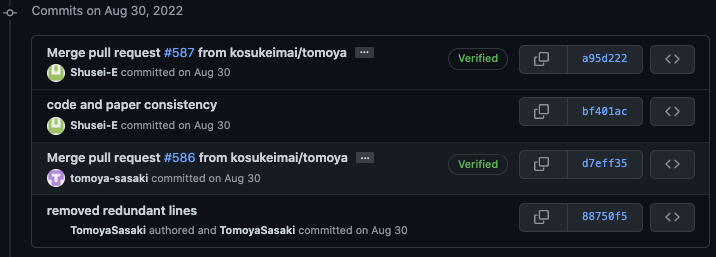
\includegraphics[width = \linewidth]{github_history.png}}
    \visible<6->{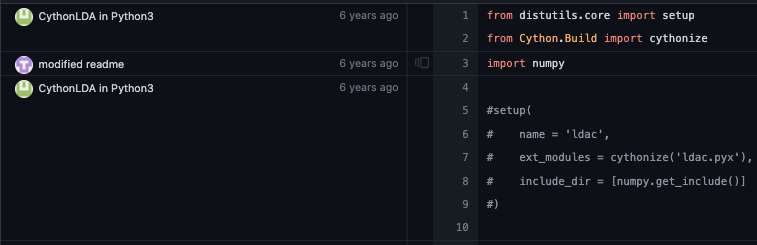
\includegraphics[width = \linewidth]{github_blame.png}} 
  \end{column}
  \end{columns}
\end{frame}

\begin{frame}{Why Git and Github: Tracking who/how/when}
  \begin{itemize}\setlength\itemsep{-3pt}
    \item You can check how the results change when we try different specification
    \item Easy to track which part of the results changed 
  \end{itemize}
  \vspace{10pt}
  \centering
  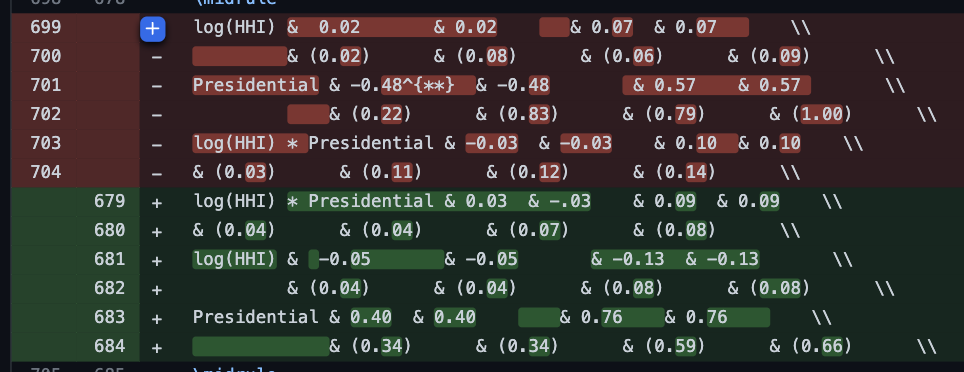
\includegraphics[width = 0.7\linewidth]{github_regression.png}
\end{frame}

\begin{frame}{Other side benefits of Git/Github}
  \begin{columns}[c]
    \begin{column}{0.46\linewidth}
      \begin{itemize}\setlength\itemsep{10pt}
        \item<1-> Hosting a customizable website (free, no ads, tons of templates)
        \item<2-> Contribute to software packages hosting on Github
        \item<3-> Tweak a package developed by someone else for your own purposes
        \item<4-> Send a request to package developer (often happens at ``Issue'')
        \item<5-> Nice integration with popular apps/websites such as Rstudio and Overleaf 
      \end{itemize}
    \end{column}\hfill
    \begin{column}{0.53\linewidth}
      % \begin{overprint}
      % \centering
      % \onslide<2-3|handout:1>{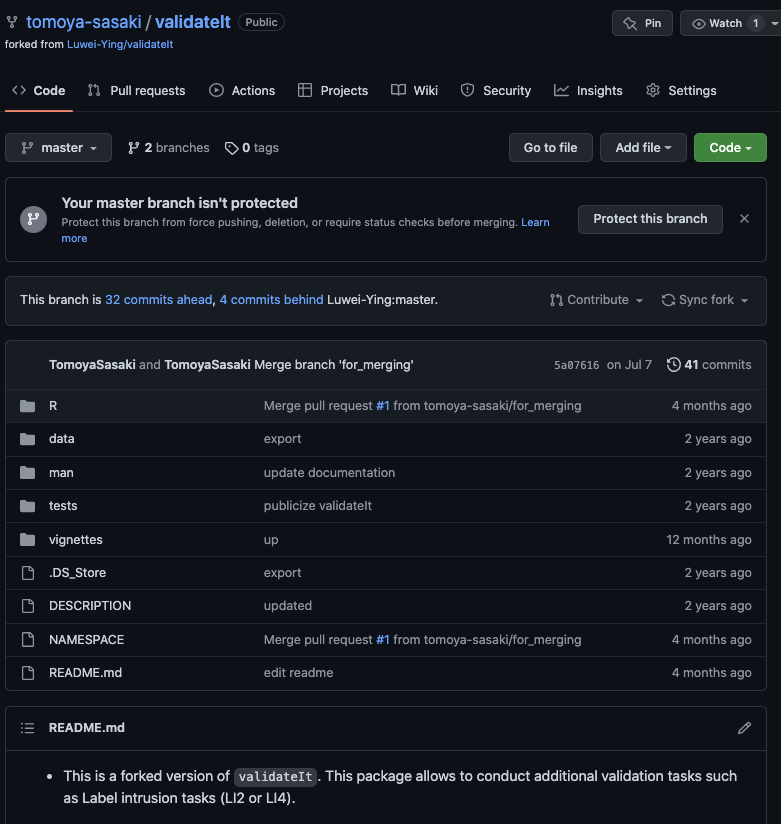
\includegraphics[width = 0.85\linewidth]{github_forked.png}}
      % \onslide<4|handout:2>{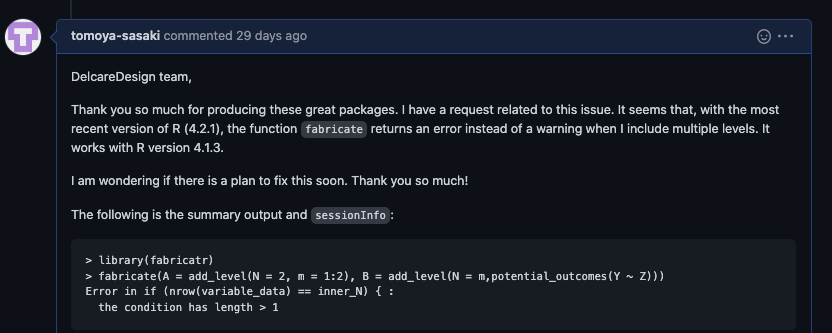
\includegraphics[width = \linewidth]{github_issue.png}} 
      % \end{overprint}
      \centering
      \only<2-3|handout:1>{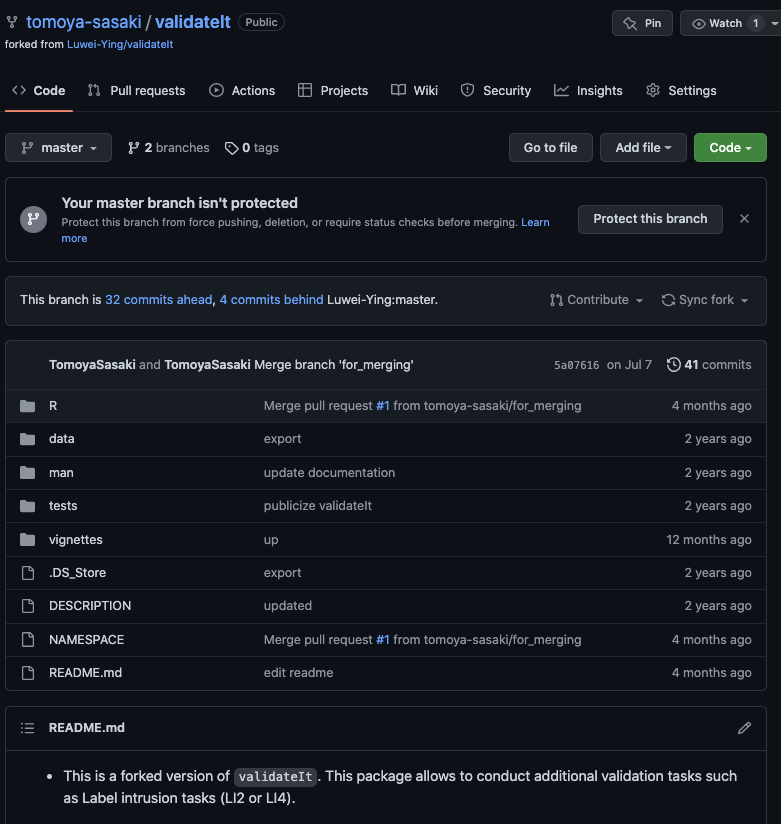
\includegraphics[width = 0.85\linewidth]{github_forked.png}}
      \only<4|handout:2>{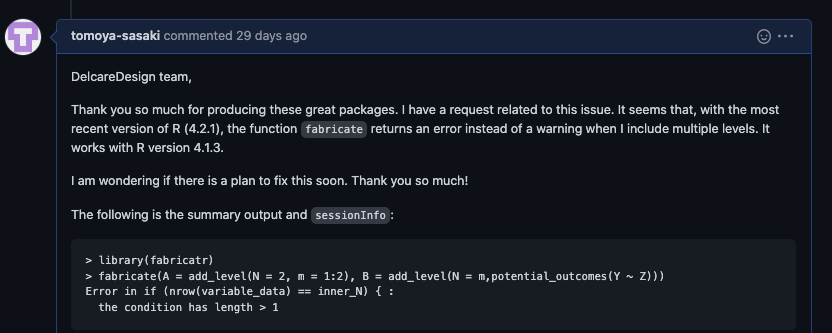
\includegraphics[width = \linewidth]{github_issue.png}} 
      \only<5|handout:3>{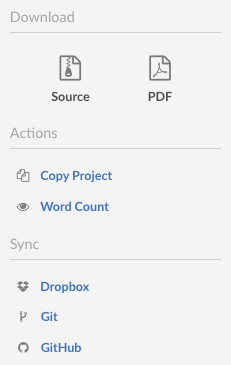
\includegraphics[width = 0.5\linewidth]{github_overleaf.png}} 
      \end{column}
  \end{columns}
\end{frame}

\begin{frame}[fragile]{Limitations: not suitable to track large files}
  \begin{itemize}
    \item Github imposes file size limits:
    \begin{itemize}
      \item 25 MB per file limit 
      (you can change this limit up to 100MB by changing setup)
      \item 1GB per repository limit
    \end{itemize}
    \item Remember that \texttt{.git} tracks and stores all the change you make in a repository
    \item[] $\leadsto$ if you store a huge file in the repository and let \texttt{.git} tracks 
    its changes, the \texttt{.git} folder can grow quite huge
    \medskip
    \item Use \texttt{.gitignore} to specify files that Git should ignore
    \begin{Verbatim}[frame=single, label=.gitignore]
      *.csv # ignore csv files
      /data/ # ignore data folder
    \end{Verbatim}
    \item Include huge files as well as sensitive files (password, API key etc) in \texttt{.gitignore}
  \end{itemize}
\end{frame}

\begin{frame}[fragile]{Limitations: not great if you want to track non-text files}
  \begin{columns}[c]
    \begin{column}{0.46\linewidth}
      \begin{itemize}\setlength\itemsep{10pt}
        \item Git cannot track line by line changes for non-text files such as 
        PDF, Microsoft Word/Excel/Powerpoint, JPG, ...
        \item Note that Git still tracks changes
        \item The value of Git/Github is limited
        \medskip
        \item In the left example, Git/Github recognizes the changes as the changes in file sizes\\
        $\leadsto$ even though you update a figure in PDF or PNG format, 
        Git/Github might not recognize it unless the file size changes...
      \end{itemize}
    \end{column} \hfill
    \begin{column}{0.53\linewidth}
      \centering
      \only<1>{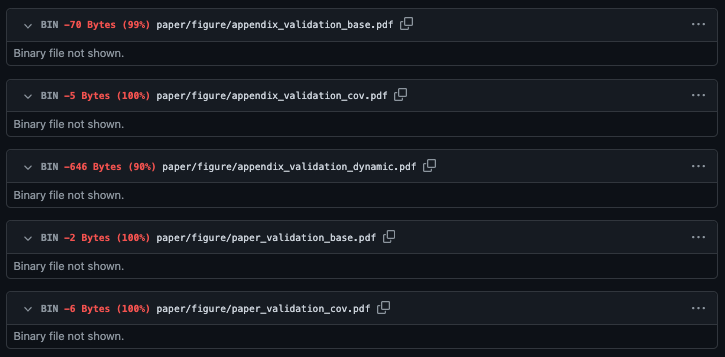
\includegraphics[width = \linewidth]{github_pdf.png}}
    \end{column}
  \end{columns}
\end{frame}

\backupbegin
\backupend
\end{document}
